\section{Design Brief and Method for the Dynamic Honeycomb Maze}



\subsection{Dynamic Honeycomb Maze Brief}
\label{section:design_brief}

\begin{figure}[h]
    \centering
    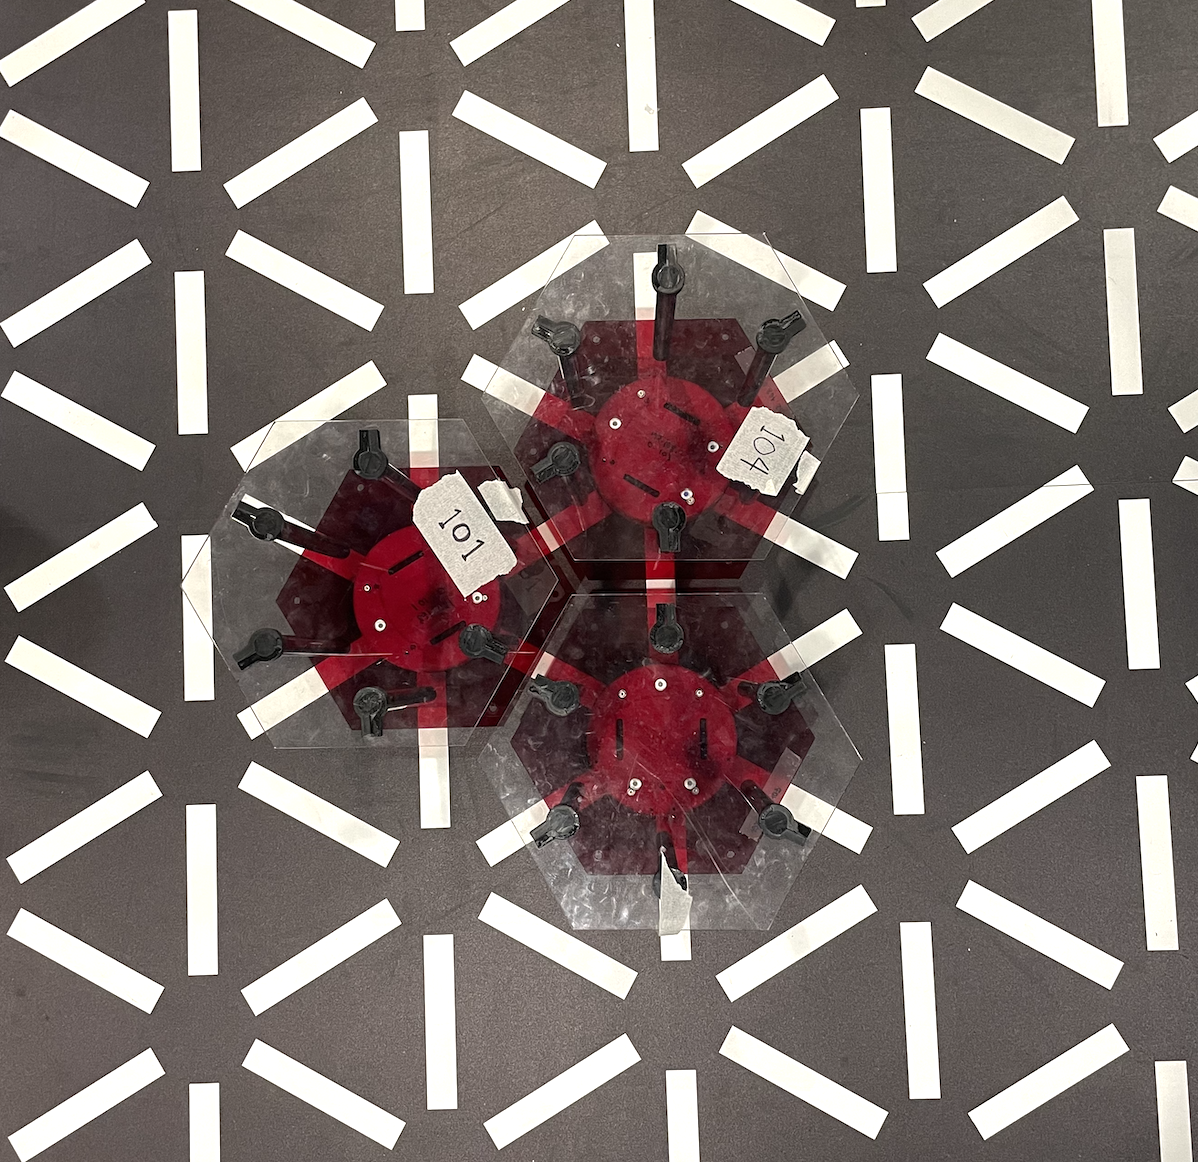
\includegraphics[scale=0.35]{images/irl_maze.png}
    \caption{This figure shows a top down view of one of the configurations of the honeycomb maze where there a hexagonal grid where the hexagonal robots are placed on top. Upon one of these platforms the animal would be placed on the hexagons and would choose which platform to move to.}
    \label{fig:picture_of_maze}
\end{figure}

There are three robots on the hexagonal grid and one has the animal placed on it. They are all placed in a room with the grid marking the floor, representing the maze that the animal traverses.

Figure is a example of a single cycle shown in Figure \ref{fig:example_algorithm}:
\begin{enumerate}
    \item(Fig. \ref{fig:example_algorithm} Panel A) The animal is placed on a robot which is adjacent to the other platforms. The animal must chose to move to either unoccupied platform. This is entirely the mouse's decision (shown in Fig. \ref{fig:example_algorithm} panel B).
    \item After the animal has moved, the remaining now-unoccupied platforms will be moved by the program such that they are positioned adjacent to the newly occupied platform (as shown in fig. \ref{fig:example_algorithm} panel C).
    \item This cycle will continue until the animal reaches the required goal.
\end{enumerate}



\begin{figure}[H]
    \centering
    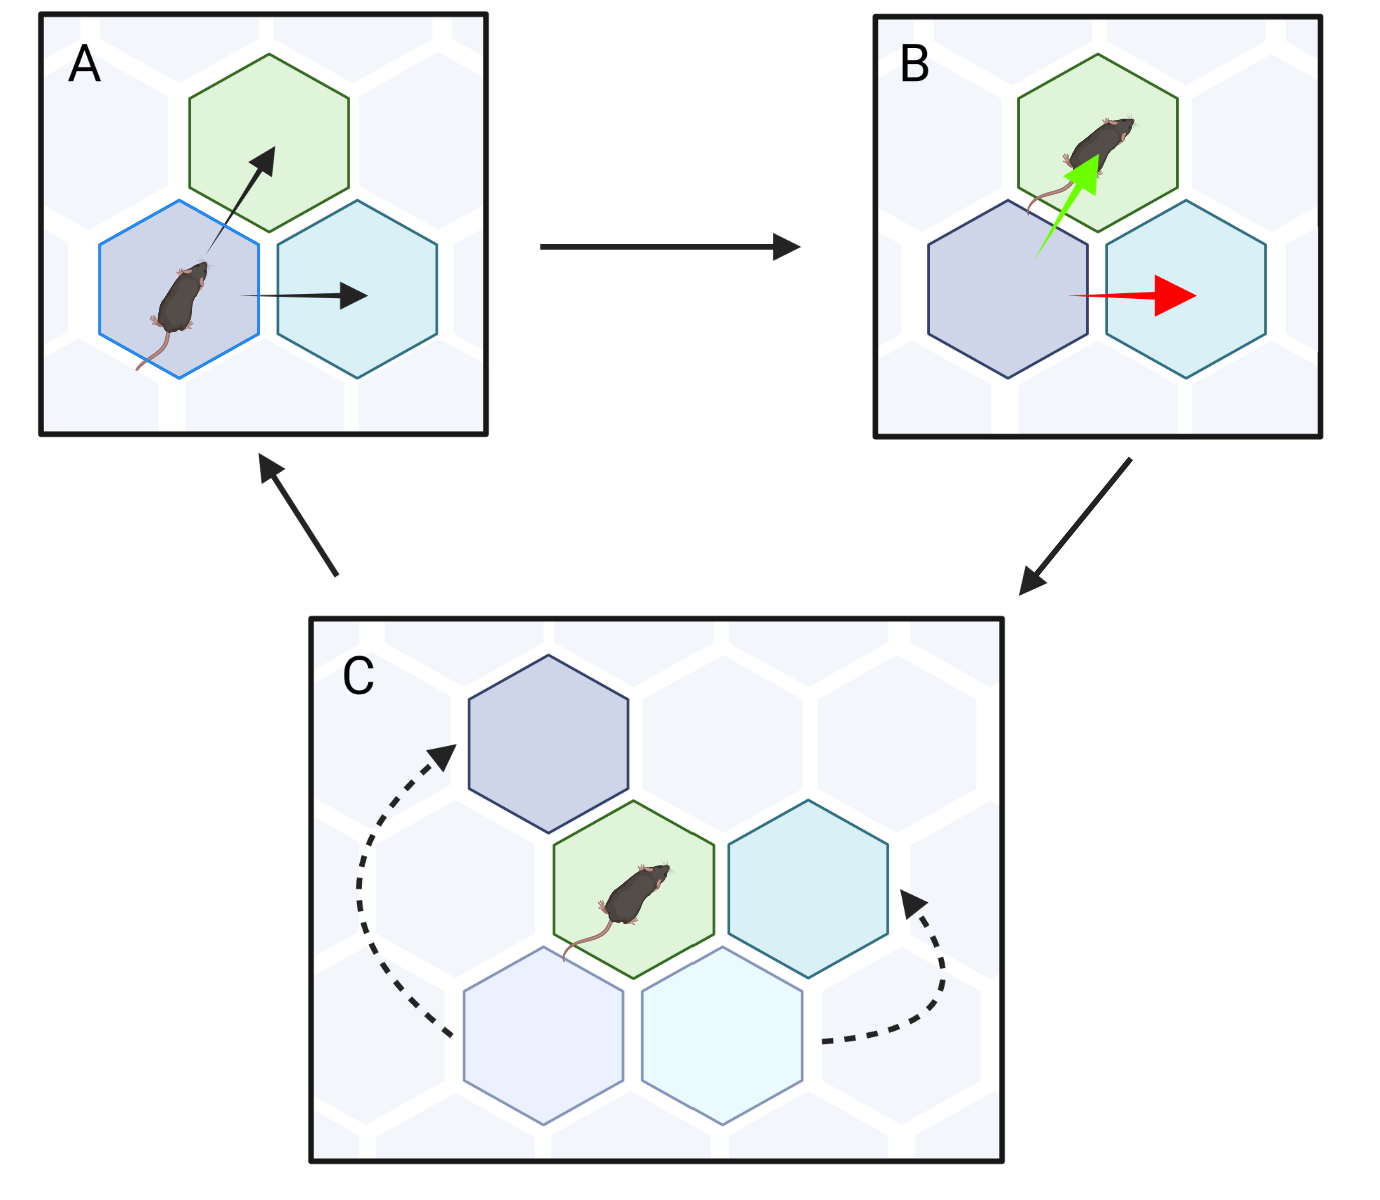
\includegraphics[scale=0.6]{images/example_algorithm.png}
    \caption{ This is a visual representation of a single cycle of the algorithm that has been developed for the Honeycomb Maze. \textbf{Panel A} shows the animal on the dark blue platform where it can choose to move to either the green or the light blue platform. \textbf{Panel B} shows that the animal has chose the green platform to move to, and the light blue platform has \textit{not} been chosen. \textbf{Panel C} shows the function of the algorithm developed; it moves the dark blue and the light blue platforms respectively to their new places around the hexagonal platform with the animal on it so that the mouse can choose which platform it will move to again. \\ \\
    Note that in this figure, Panel C, the arrangements of the hexagons around the central green platform are examples only. They can be placed anywhere around the central green platform as shown in panel C of this figure.}
    \label{fig:example_algorithm}
\end{figure}


\subsection{Hexagonal Grid and \textit{Khepera IV} Robots}
% Section about the grid upon which the robots are placed

On the floor of the experimentation room a hexagonal grid is printed (Fig. \ref{fig:hexgrid_with_numbers}). The lighter lines are detected by infra-red sensors on the bottom of the robots \ref{fig:robot} and used to calculate the distance or angle rotated or translated across the grid.

\begin{figure}[h]
    \centering
    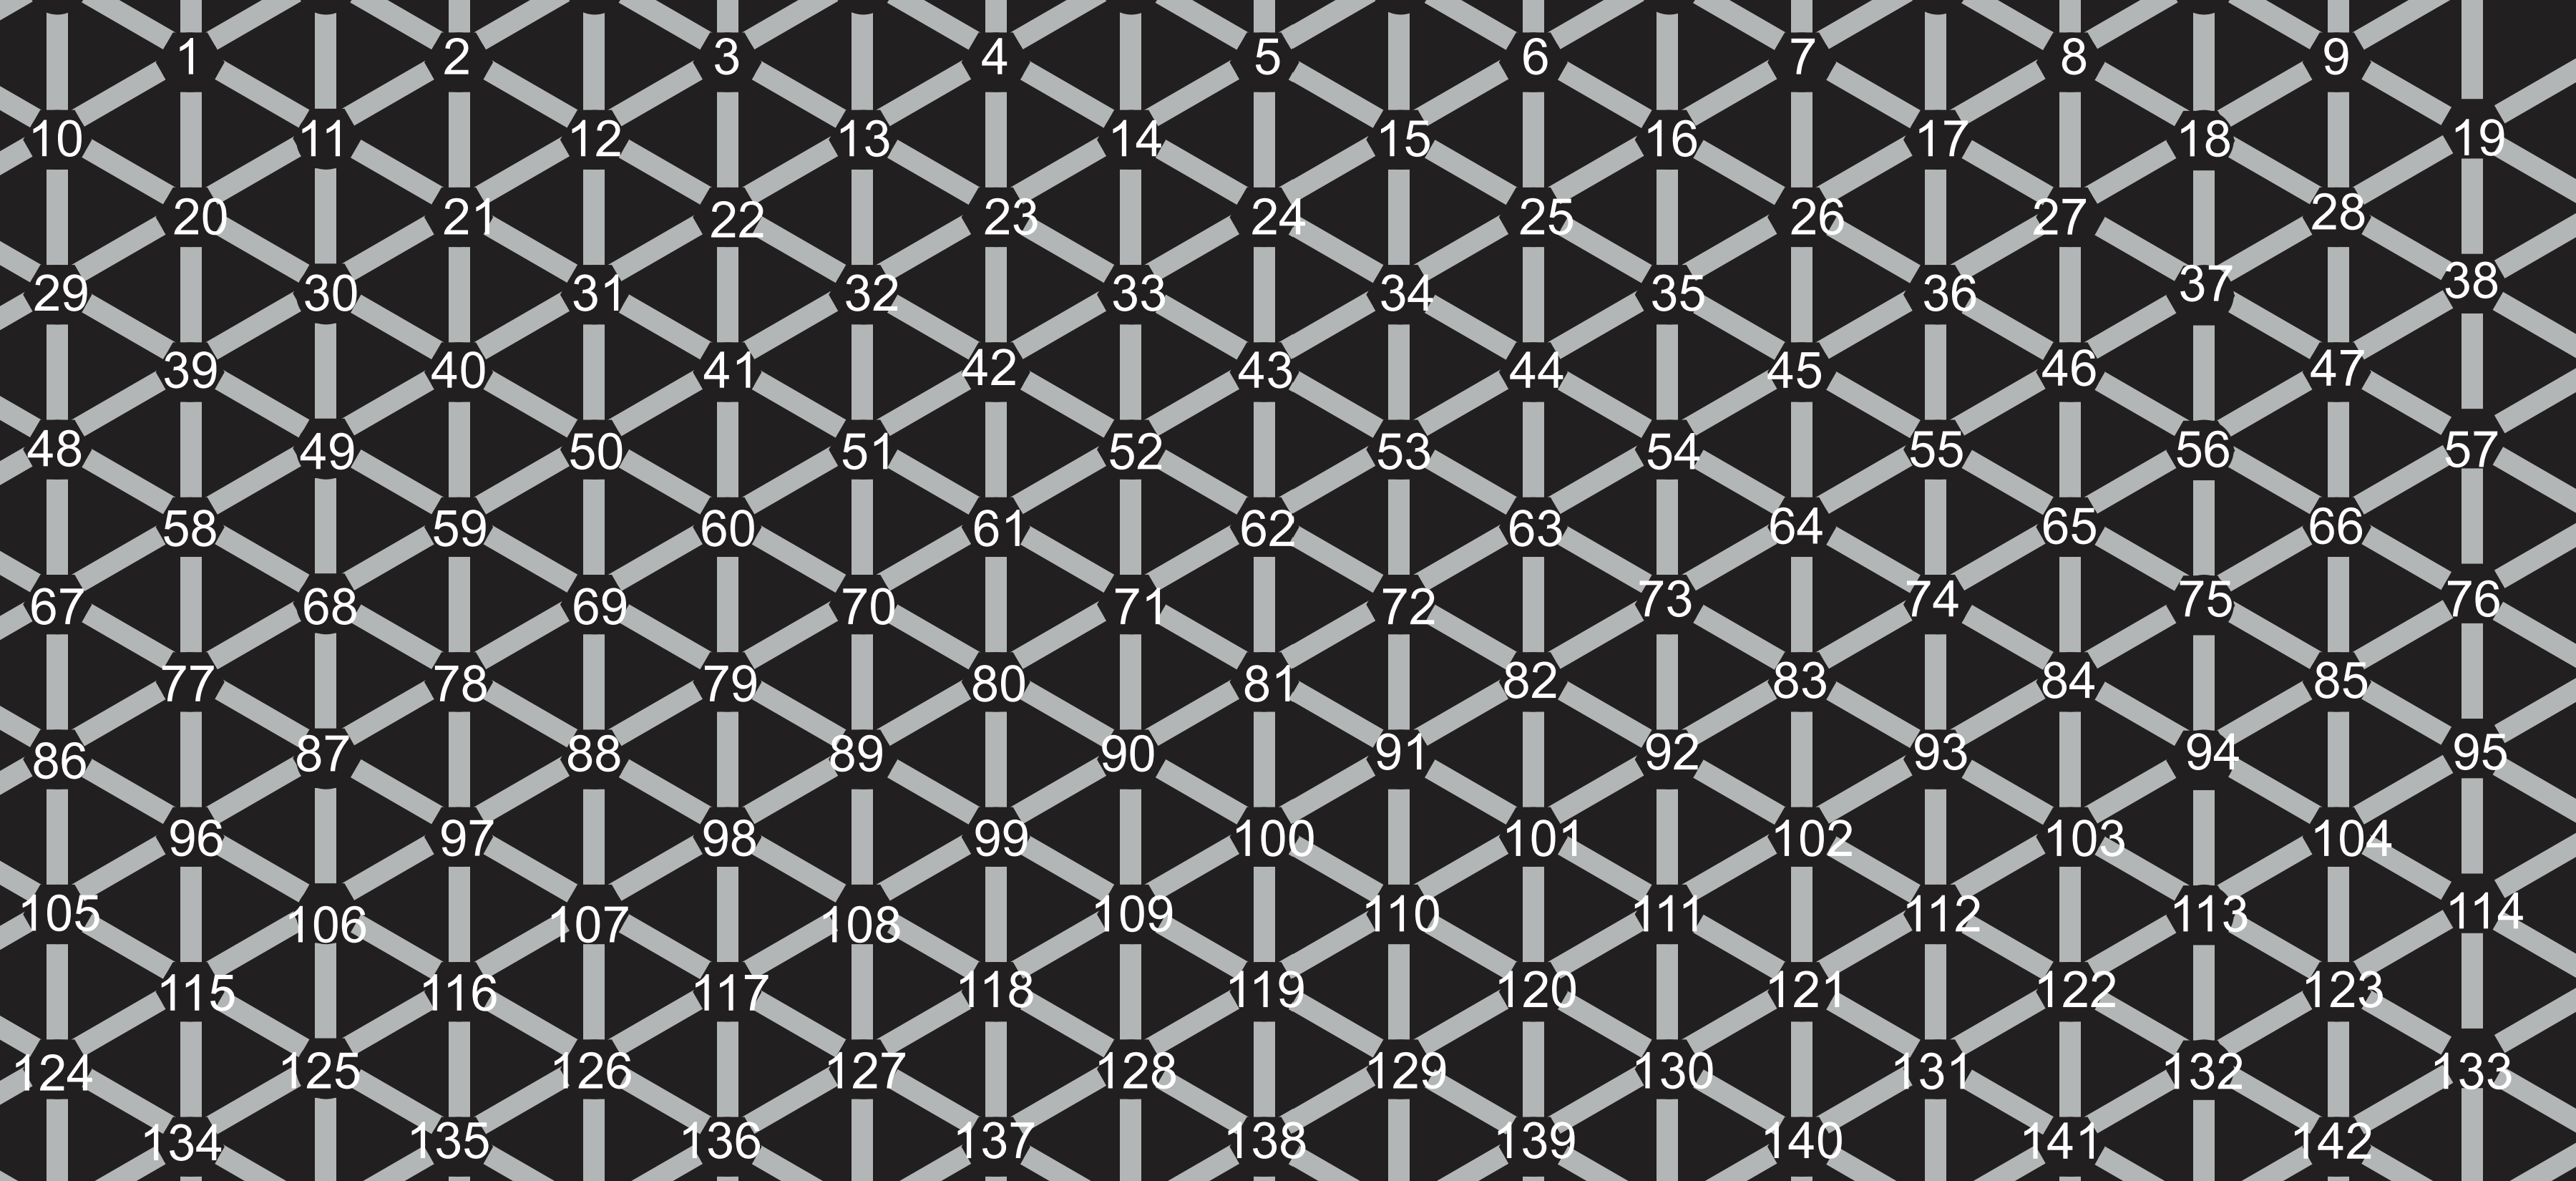
\includegraphics[scale = 0.3]{images/hexgrid_with_numbers.png}
    \caption{This shows the mat on the floor of the experimentation room which the line following robots will navigate. The black and light grey lines can be detected by the line following robots' IR sensors.}
    \label{fig:hexgrid_with_numbers}
\end{figure}


% Section about the Khepera IV robot, their design and hence the limitations

The robots used in this maze are the \textit{Khepera IV} robots (see Fig. \ref{fig:robot}). On their bottom surface, they have IR sensors allowing them to detect when they have passed over a light grey line. 
This allows them to keep track of the number of rotations they have made in place or the number of translations they have made, allowing reliable navigation around the hexagonal space.

Due to the parallel arrangement of the wheels on the robots, they are only able to move forwards or backwards or turn in place. In order to alter the direction of travel, the robots must first rotate \textit{and then} translate.

The program has been written in Python 3. Following the animals movement, the program makes a decision, computes a set of commands which are then sent to the robot via an SHH protocol. They will then be executed (See Appendix \ref{fig:integration_network}).

\begin{figure}[h]
    \centering
    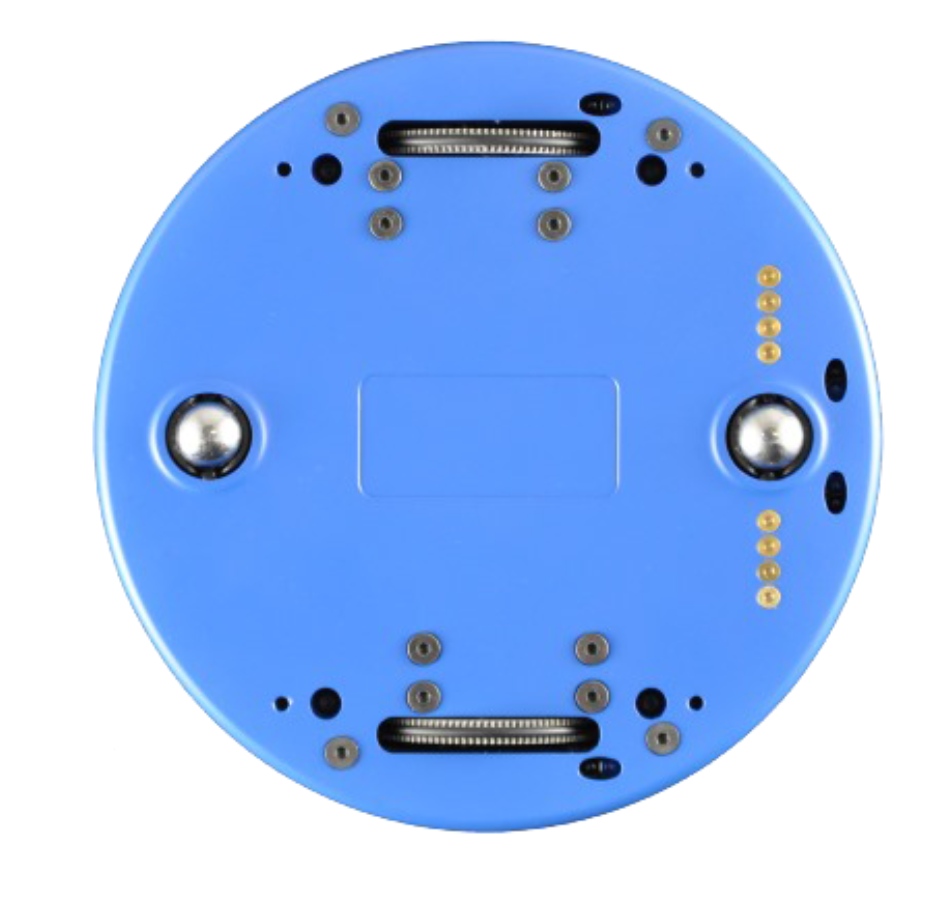
\includegraphics[scale = 0.5]{images/khepera_IV_robot.png}
    \caption{Shown is the underneath of the \textit{Khepera IV} robot. Note the presence of the 2 parallel wheels of the robot. 
    Whenever the platform robot wants to move to the out of its current direction of travel, it must first rotate to its desired direction of travel and then translate forwards.
    This leads to significant movement limitations of the \textit{Khepera IV} robots which must be addressed in the development of the program to control the Dynamic Honeycomb Maze. \\ \\
    }
    \label{fig:robot}
\end{figure}

\subsection{Platforms}

%Section about the design of the platforms of the robot and the limitations that come with it
% Due to the hexagonally tiled space,  consecutive tiles cannot rotate next to each other, otherwise they will collide.

The geometry of the hexagonal grid prevents adjacent robots from rotating directly next to each other as they will collide (Fig. \ref{fig:collision}).

\subsection{Summary of limitations of the line following robot and its platform.} 

Below are the intrinsic design constraints that the program must overcome for a successful Honeycomb Maze to be developed:
\begin{tcolorbox}
\begin{enumerate}
\item To avoid collisions, a robot cannot be adjacent to another robot when they rotate as they are hexagonal-shaped. 
% \item Two hexagonal robots \textit{that are adjacent} are unable to rotate without colliding. To avoid this, a robot cannot be adjacent to another robot when they rotate (see Fig \ref{fig:collision} for example collision).
\item The robots have a sense of polarity since their wheels are parallel. This means they cannot change direction without rotating first.
\end{enumerate}
\end{tcolorbox}

% These design constraints result in a limited range of movement of the robots when they are consecutive to each-other and can only move without restrict when not

% This results in a limited range of movement of the platforms when they are consecutive to each other and are in fact only able to move without restriction when they are not consecutive to any other platform robots.